\documentclass[10pt]{article}
 
\usepackage[margin=1in]{geometry} 
\usepackage{amsmath,amsthm,amssymb, graphicx, multicol, array}
\usepackage{enumitem}
\usepackage{hyperref}
 
\newcommand{\N}{\mathbb{N}}
\newcommand{\Z}{\mathbb{Z}}
 
\newenvironment{problem}[2][Problem]{\begin{trivlist}
\item[\hskip \labelsep {\bfseries #1}\hskip \labelsep {\bfseries #2.}]}{\end{trivlist}}

\date{Due: Nov 9, 2022 10pm PT}

\begin{document}
 
\title{Assignment 7}
\author{
CS 181AG: Network Algorithmics}
\maketitle

This assignment will help you understand details of the iSLIP algorithm, Network Address Translation, and TCP. 

\begin{problem}{1: Motivating the iSLIP pointer increment rule}
Let's explore why updating the pointer after each iteration could lead to unfairness in iSLIP. Consider a situation where we have three inputs, A, B, and C, and three outputs, 1, 2, and 3. A always has traffic for 1, 2, and 3 (i.e., its queues for those ports are endless). B and C always have traffic for 2. 

\begin{enumerate}
    \item Draw the scenario as we did in class, but update the grant pointer and accept pointer after \emph{each iteration}, rather than only after the first iteration in each round. You should draw enough rounds to show that traffic can be continually starved between a particular input-output port pair. Please draw each round and iteration separately, showing the grant and accept steps for each (because request is the same each time). Label both the round and iteration as well as where the grant and accept pointers are at each step. Which port pair is starved?
    
    \item Now draw the same scenario as above but using iSLIP correctly. That is, in each round, the grant and accept pointers are updated only after the first iteration. Similarly, draw the grant and accept steps for each round and iteration, along with the grant and accept pointers. Draw enough rounds to show that each port pair gets a chance to connect. 
\end{enumerate}
\end{problem}
\subsection*{Answer 1:}
\begin{enumerate}
    \item We can see that we have the first 3 rounds of our modified iSLIP pointer increment rule. Looking at the results of these rounds, we can see that the port pair that is starved is the pair $(A,2)$.
    \begin{center}
        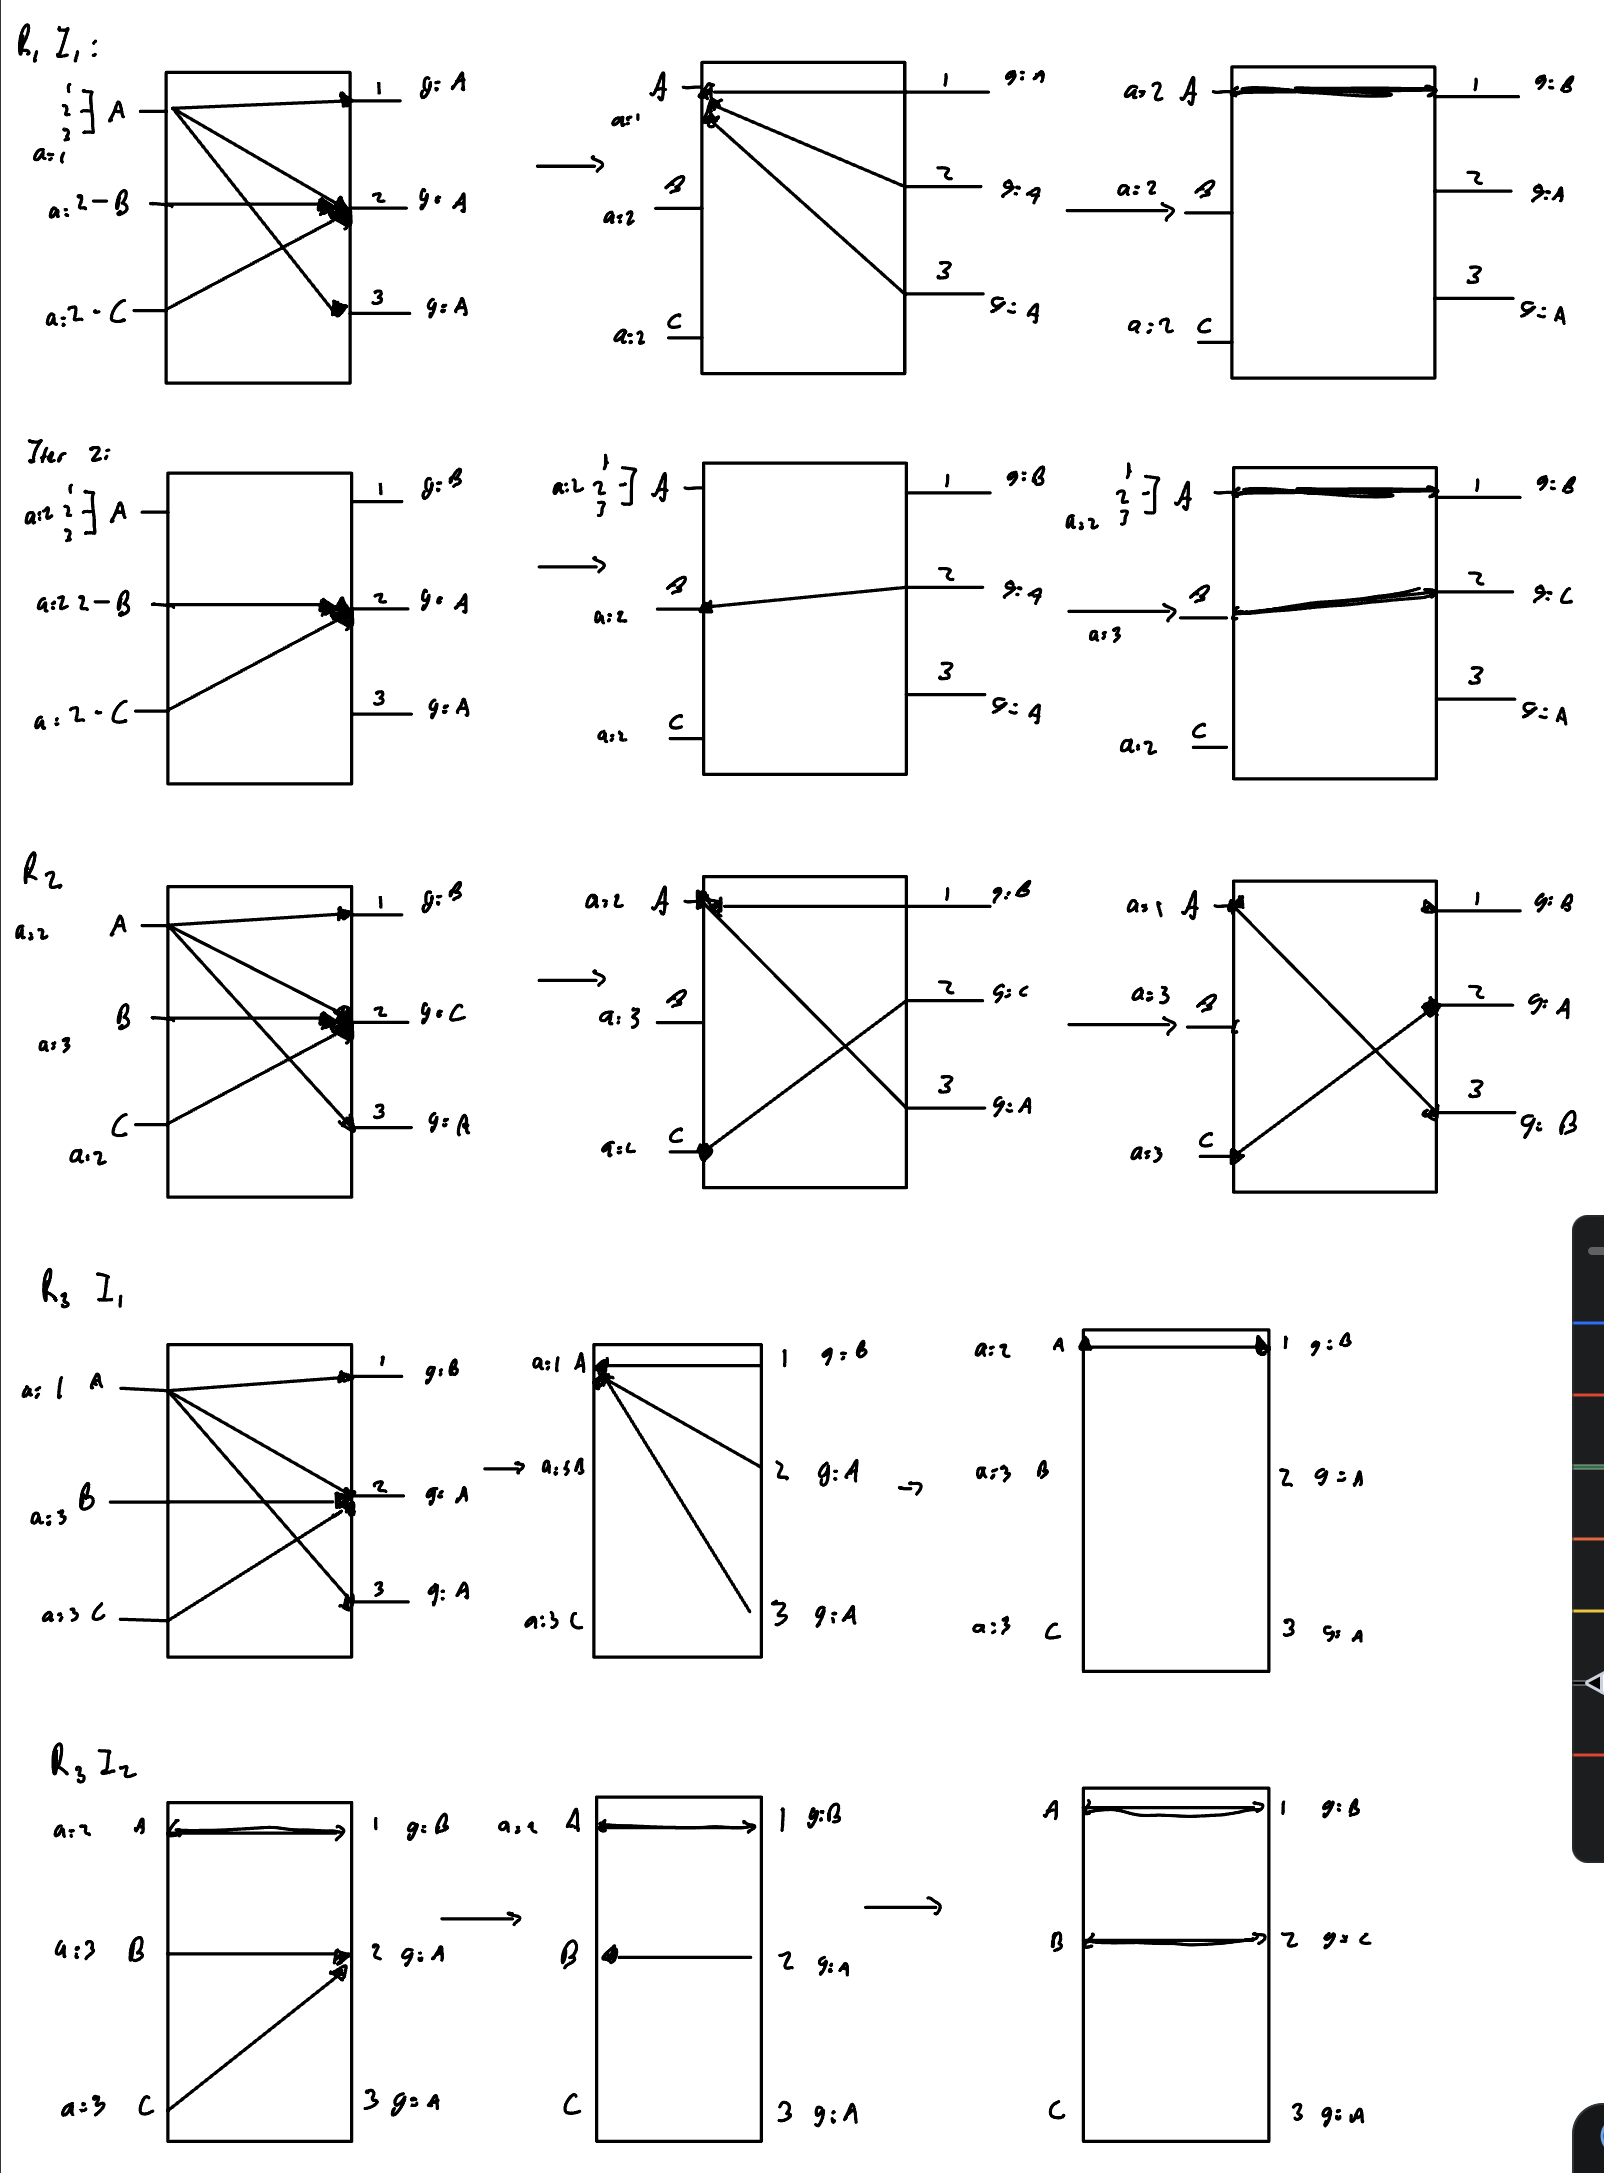
\includegraphics[scale = 0.25]{hw7pr1a.jpeg}
    \end{center}
    \item Now, we can draw the same scenario with iSLIP being used correctly as follows,
    \begin{center}
        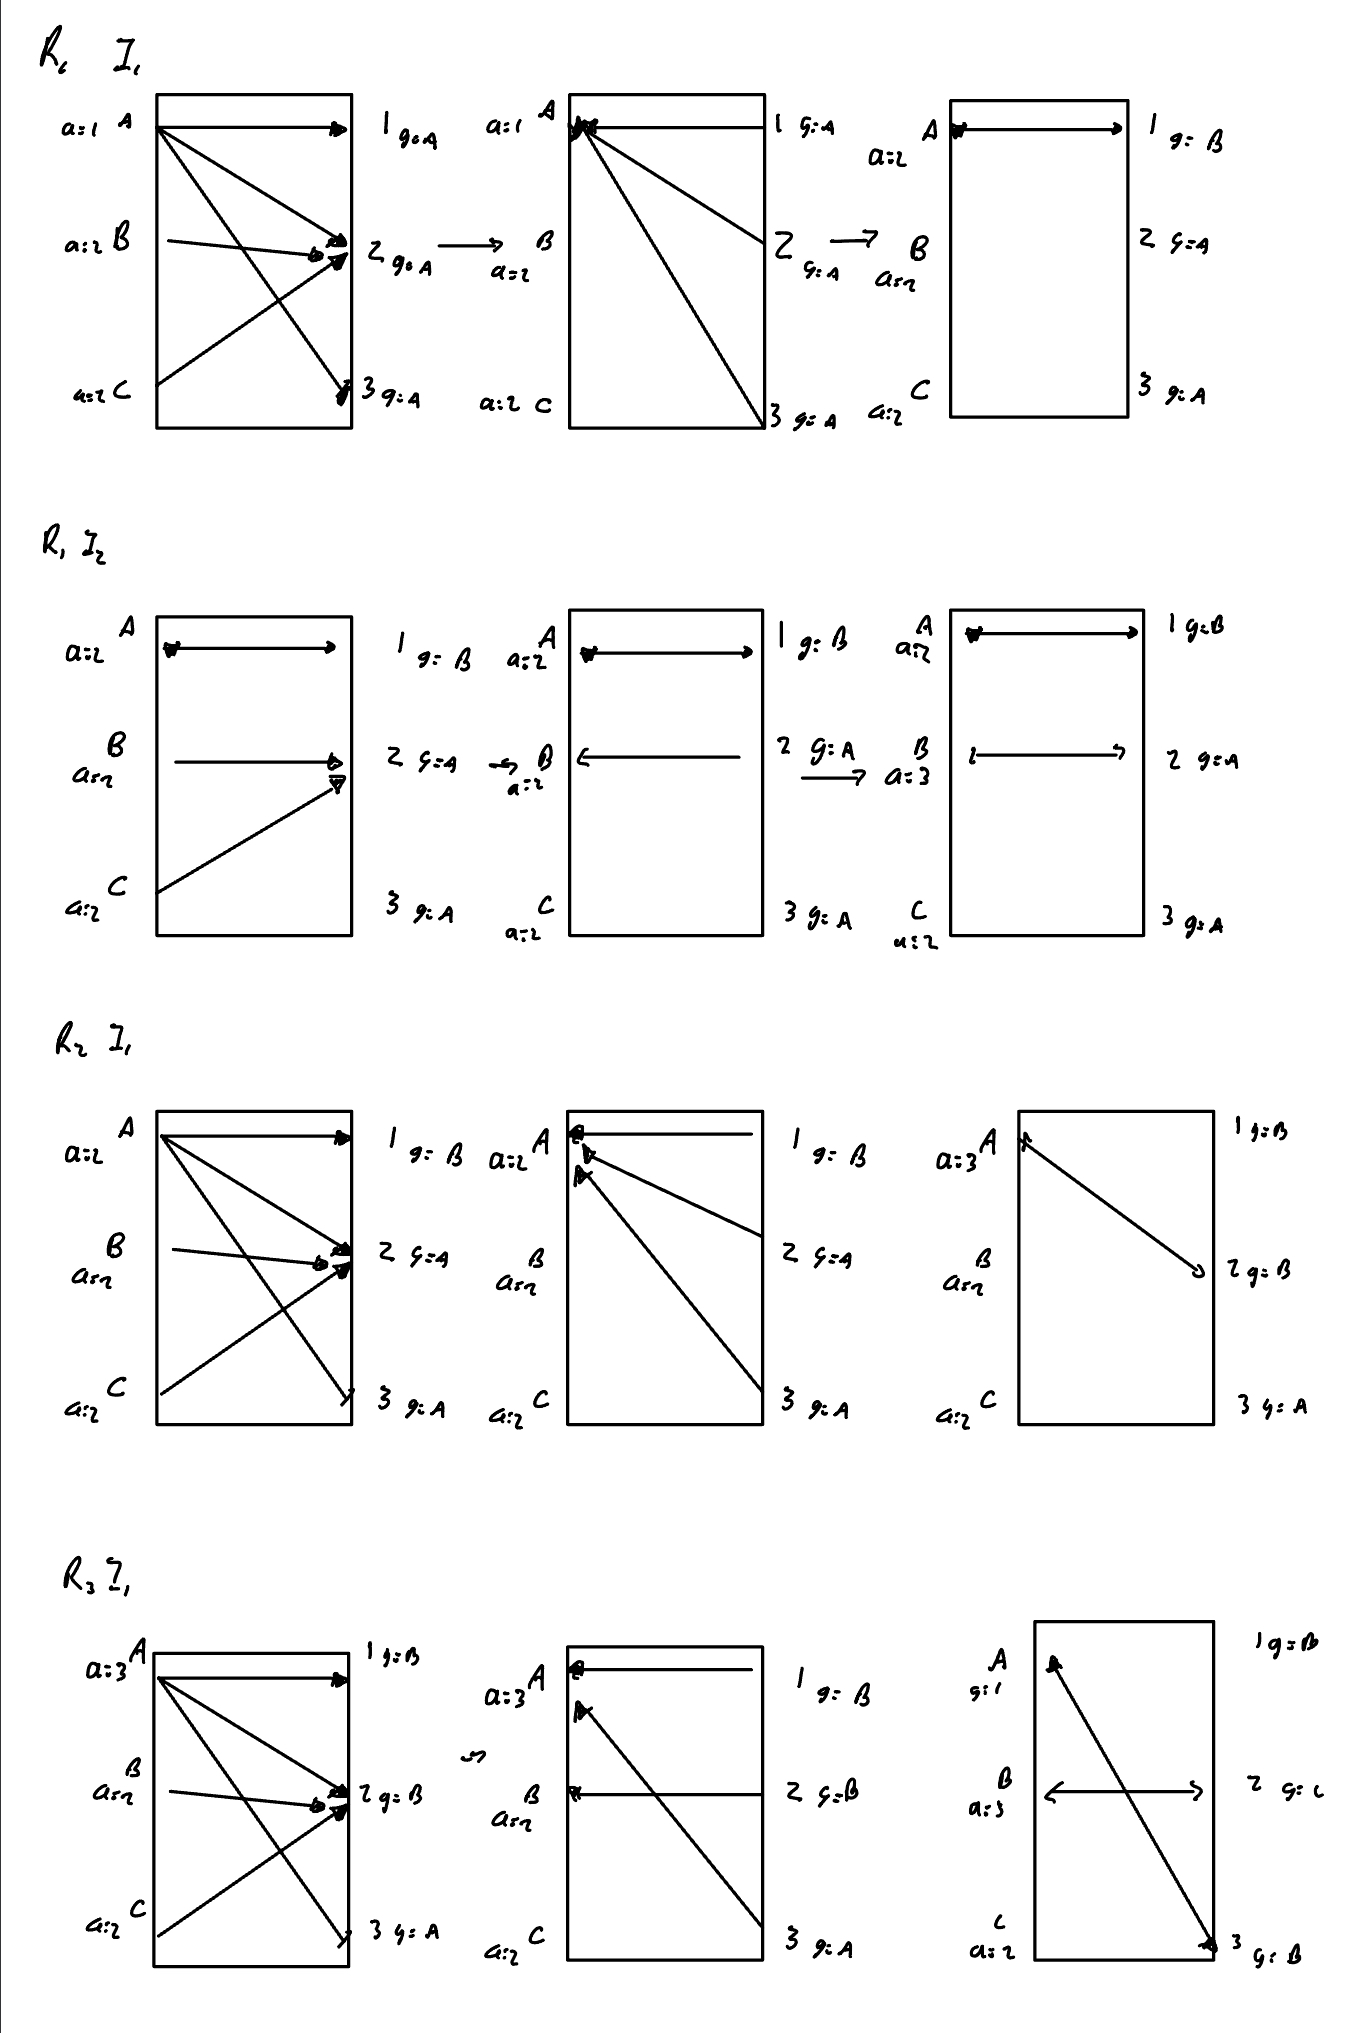
\includegraphics[scale = 0.35]{hw7pr1b1.jpeg}
        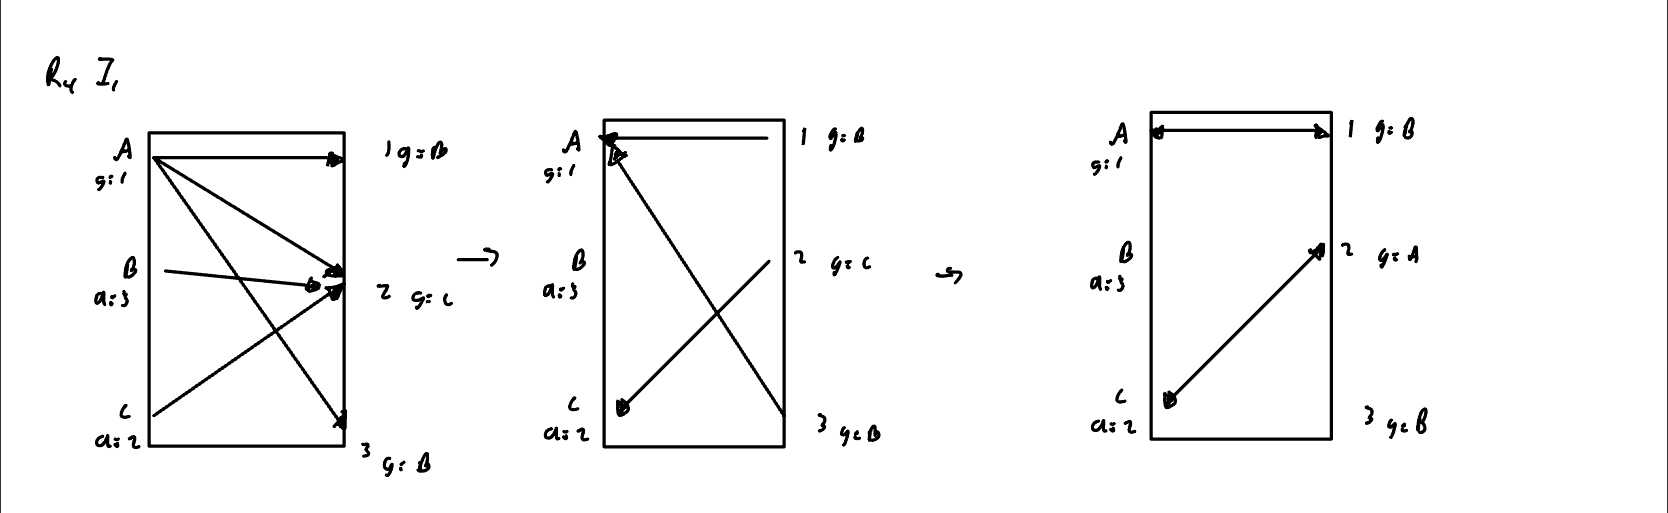
\includegraphics[scale = 0.3]{hw7pr1b2.jpeg}
    \end{center}
\end{enumerate}


\begin{problem}{2: Network Address Translation}
In the example of NAT we looked at in class, the router sees a packet from a device in the network with IP address 192.168.1.2 (a private address) and source port 17534. It is destined for 8.8.8.8:80, as the device user would like to browse Google. The router then changes \emph{both} the IP address and the source port. It changes the IP address to the network's public IP address and it generates a new source port. 

We have discussed how having public vs. private IP addresses is beneficial for the IP address shortage, but why must the router also change the source port?
\end{problem}
\subsection*{Answer 2:}
The reason why the router must also change the source port by generating a new source port in order to ensure that the packet coming back from the destination IP address ends up going to the correct device on the private IP address. That is, by generating a new source port for every device that lives within the network and wants to send a message to a device outside of the network, the router can keep track of where a packet came from so that way it can forward any response packets to the right private IP addresses, thus creating a mapping betweent the source ports on the router and the private IP addresses within the network as a way to distinguish between devices within the network while still using the public IP address of the whole network.
\begin{problem}{3: Sliding Window Protocol}
Assume that a sender would like to send 10 packets to a receiver, each with size = 1 byte, starting with sequence number 0. The window size is 3, and the network is such that every 5th data packet is lost (but no ack packets are lost), including both original transmissions and any necessary retransmissions. Also assume that if the sender successfully sends a packet at time \emph{t}, it will receive an ack packet at time \emph{t}+3. The sender can send one packet at each time slot, and if it was waiting on an ack packet before sending, it can send in the same slot that it received the ack, i.e., there is no processing time at the sender. 

The first packet of this scenario is shown below. Show the rest of the communication, drawing the sequence number every time the sender sends a packet and the ack number every time the receiver sends an ack. You can represent lost packets by a link that does not reach the receiver. You do not need to include the size like we did in class because it is always 1 byte. Many time slots are provided to you, but you do not need to use all of them. 

\begin{figure}[h!]
    \centering
    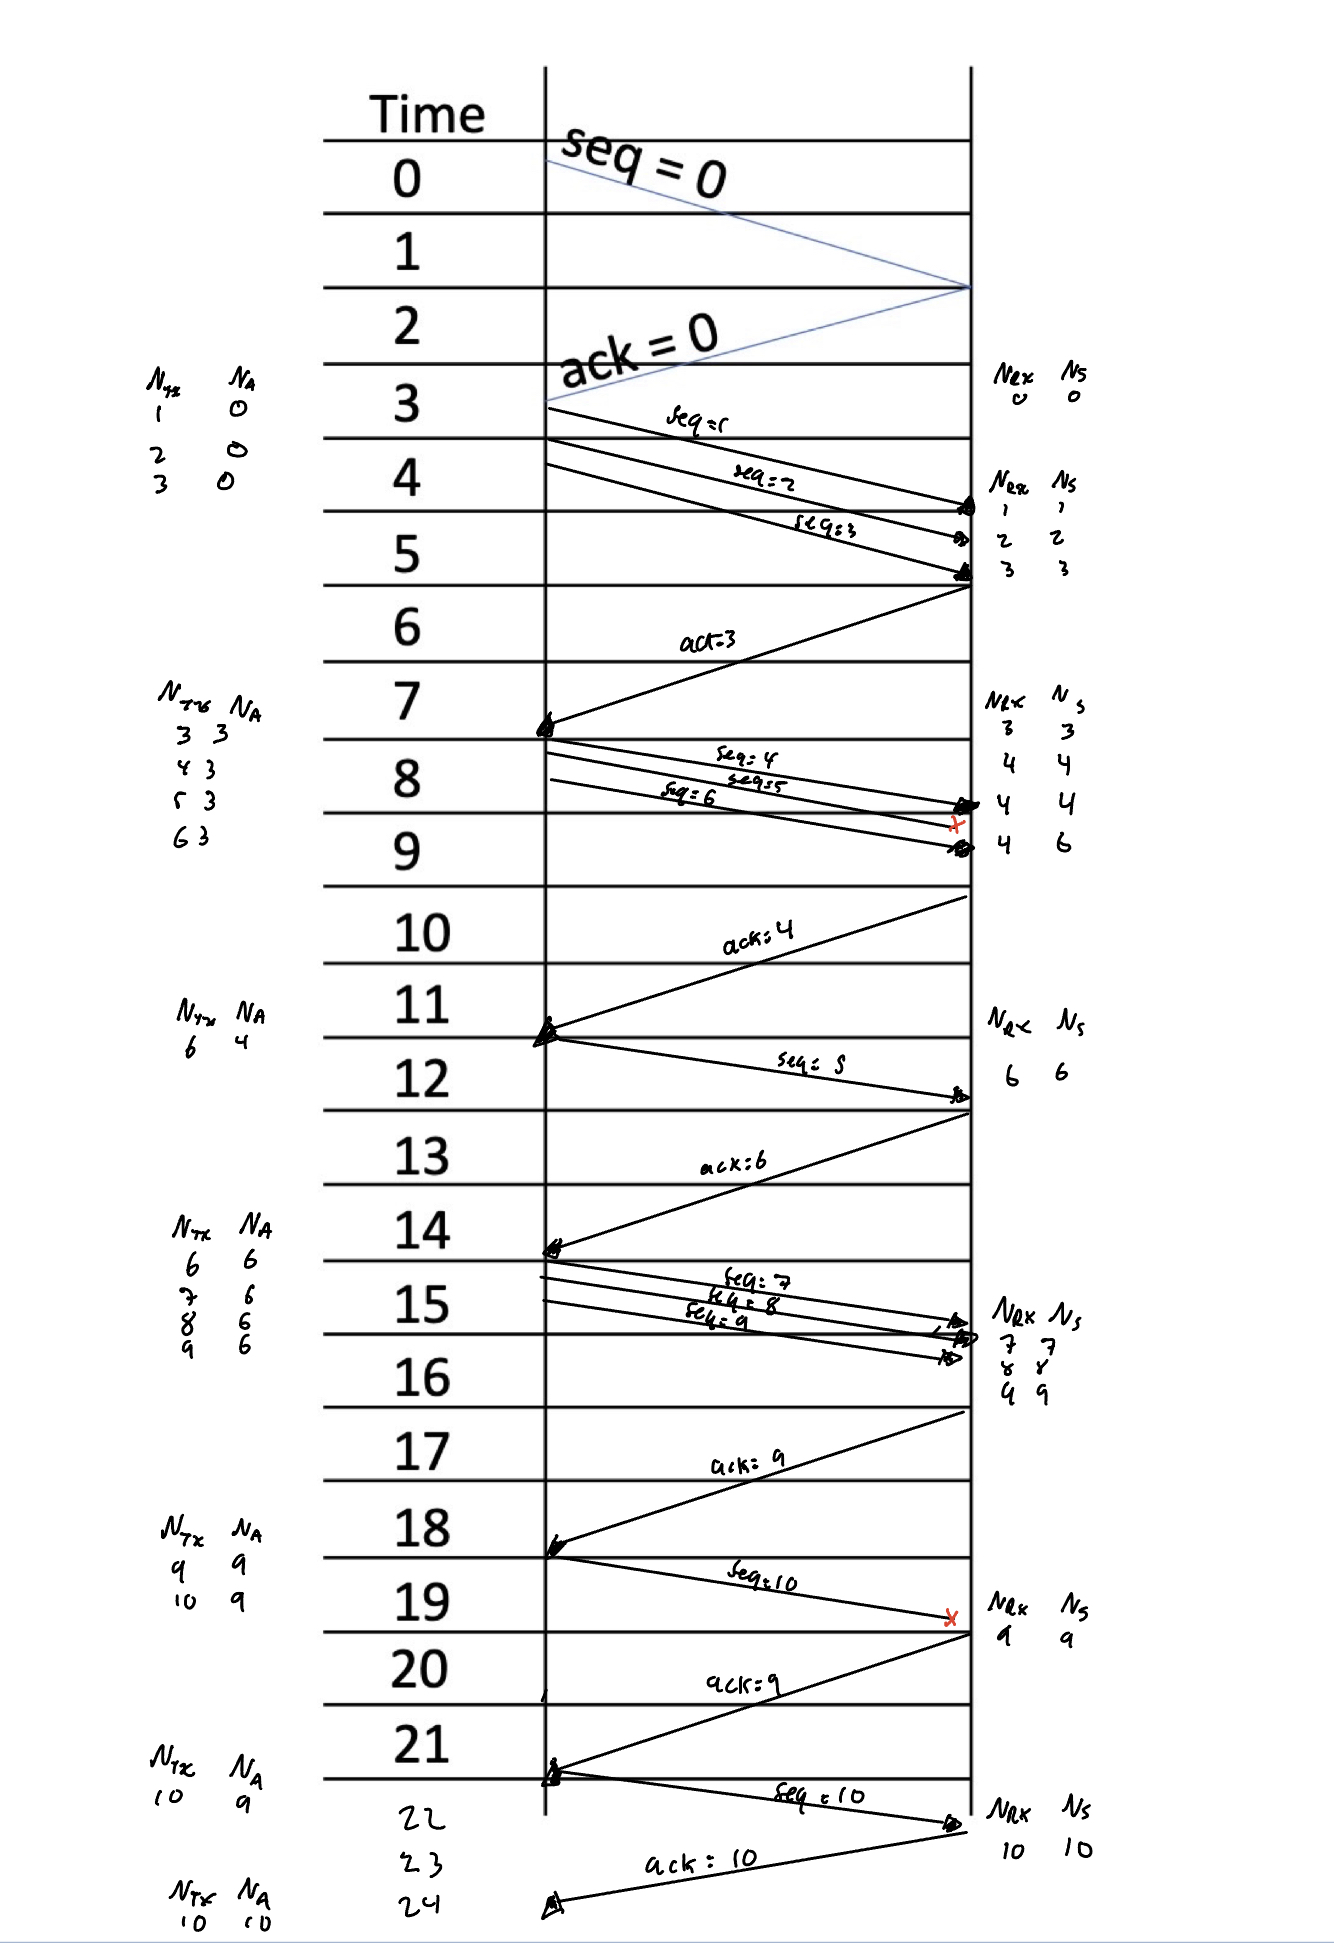
\includegraphics[scale = 0.25]{hw7pr3.jpeg}
\end{figure}

\end{problem}
\newpage
\begin{problem}{4: Reading}
In class, we've learned about many algorithms that are built into hardware to make the router's various jobs run faster. While hardware continues to be the faster option (by a lot), it lacks flexibility and delays the possibility of updating to new algorithms. Read \href{https://cs.nyu.edu/~anirudh/domino-sigcomm.pdf}{this} this paper about one attempt to add this flexibility. Then answer the following questions:

\begin{enumerate}
    \item What are the main benefits and challenges of programmable switches?
    \item What is the key problem this paper tries to solve? Why is it a hard problem?
\end{enumerate}
\end{problem}
\begin{enumerate}
    \item The main benefits of programmable switches are that they are reconfigureable based off the choice of software, "field reconfigureable", and allow programmers to program different protocols (such as packet parsing and forwarding) such that "the set of protocol formats to be matched and the set of actions to be executed when matching packet headers in a match-action table", thus making the actual match-action processing expressable independently of the hardware. Some of the challenges of programmable switches are that for different algorithms, the programs must write the algorithms in a manner that is independent of different hardware components which is more difficult, such as for different devices such as routers, network processors, and network endpoints.
    \item The key problem this paper tries to solve is the problem pertaining to the rigidity of data-plane algorithms when trying to run them at line rate. Traditionally, these algorithms have to be programmed into hardware, which means that algorithms cannot be modified or new ones installed. This is a challenging problem to answer due to the fact that, according to the article, "many data-plane algorithms create and modify algorithmic state", which thus makes it difficult to achieve line-rate programmability, due to the sequentiality of hardware but also the actions of different bits of hardware with modifying different atomic states.
\end{enumerate}
\begin{problem}{5}
How long did this assignment take you?
\end{problem}
\subsection*{Answer 5:}
This assignment took me $\approx 5$ hours.
\end{document}


